\section{Air pollution - sources and behaviour}
\label{sec:whatisairpollution}

\subsection{What is air pollution?}
\label{subsec:whatisairpollution}
Air pollution is defined by \cite{colls1997} as "material emitted into the air from stationary or mobile sources, moving subsequently through an aerial path and perhaps being involved in chemical or physical transformation before eventually being returned to the surface". This research focuses on the places in which humans, particularly in urban environments, are exposed to this pollution.

%%%%%%%%%%%%%%%%%%%%%%%%%%%%%%%%%%%
%%% PARTICLE TYPES AND SIZES
%%%%%%%%%%%%%%%%%%%%%%%%%%%%%%%%%%%

\subsection{Particle types and sizes}
\label{subsec:particletypesandsizes}

Air pollution is a summary term for many sub-categories of pollutants. Pollutants can be solid particles, liquid particles, or gaseous material. They can also be classified as either a primary or secondary pollutant. For example fumes emitted from the stack of a power station are classified as primary pollutants, whereas ground level ozone formed by chemical reactions between primary pollutants catalysed by sunlight are classed as secondary pollutants. The UK Department for Environment, Food and Rural Affairs (\gls{defra}) is 3 hours behind summarises the main constituents of air pollution and their typical sources as follows (\cite{DEFRA2011}):

\begin{itemize}
\item Particulate matter
\begin{itemize}
\item Combustion (traffic or stationary sources), sea-spray, construction, quarrying.
\end{itemize}
\item Oxides of nitrogen (\gls{nox})
\begin{itemize}
\item Combustion. Road transport, electrical supply industry, other industry.
\end{itemize}
\item Ozone (\gls{o3})
\begin{itemize}
\item A secondary pollutant, not emitted directly from human-made sources, but formed as a result of reactions between other pollutants (Oxides of nitrogen, volatile organic compounds) in sunlight.
\end{itemize}
\item Sulphur dioxide (\gls{so2})
\begin{itemize}
\item Combustion of fuels such as coal and heavy oils by power stations.
\end{itemize}
\item Polycyclic aromatic hydrocarbons (\gls{pahs}) 
\begin{itemize}
\item Many different sources. \gls{defra} uses Benzo[a]pyrene as a marker. Main sources are coal and wood burning, fires, industrial processes. Traffic combustion (diesel in-particular) is a major contributor.
\end{itemize}
\item Benzene
\begin{itemize}
\item Domestic and industrial combustion and road transport.
\end{itemize}
\item 1,3-butadiene
\begin{itemize}
\item Combustion of petrol i.e. motor vehicles that use petrol as a fuel source
\end{itemize}
\item Carbon monoxide (\gls{co})
\begin{itemize}
\item Occurs from incomplete combustion of fuels that contain carbon. Road transport, residential combustion and industrial combustion are the main sources.
\end{itemize}
\item Lead (Pb)
\begin{itemize}
\item Combustion of coal and nonferrous metals
\end{itemize}
\item Ammonia
\begin{itemize}
\item Mainly from agriculture such as manure, fertilisers and slurry.
\end{itemize}
\end{itemize}

When discussing the amount of pollutants in the air, either volumetric or gravimetric units are used. Volumetric units quantify the ratio of volume of pollutants to clean dry air ( itself a mixture of nitrogen, oxygen, argon etc. ), whereas gravimetric units  quantify the mass of the material per volume of air. Most laws and guidelines, such as the European Union Air Quality Standards (see Section \ref{sec:healtheffects}), use gravimetric measurements. Table \ref{tab:pollution_units} summarises the abbreviations for volumetric and gravimetric units which are used throughout this research.

\begin{table}[H]
\caption{Abbreviations for volumetric and gravimetric pollutant units}
\centering
    \begin{tabular}{ | l | l |}
    \hline 
     \textbf{Volumetric} & \\ \hline
     \textbf{Description} & \textbf{Notation} \\ \hline
      Parts per million of pollutant per parts of air volume & (10\textsuperscript{-6} ppm) \\ \hline
     Parts per billion of air pollutant per parts of air volume & (10\textsuperscript{-9} ppb) \\ \hline
     Parts per trillion of air pollutant per parts of air volume & (10\textsuperscript{-12} ppt) \\ \hline
     \textbf{Gravimetric} & \\ \hline
     \textbf{Description} & \textbf{Notation} \\ \hline
     milligrams of pollutant per cubic metre & (mg/m\textsuperscript{3}) \\ \hline
     micrograms of pollutant per cubic metre & ($\mu \text{g m}^{-3}$) \\ \hline
     nanograms of pollutant per cubic metre & (ng/m\textsuperscript{3}) \\ \hline
    \end{tabular}
\label{tab:pollution_units}
\end{table}
 
Of the ten pollutants listed above, over half list transport combustion as being a source. When combined with proximity to humans in urban environments it is easy to see why air quality in towns and cities, and in particular the pollutants caused by vehicles in these environments, receives such great interest in the field of air quality research and environmental science.

%%%%%%%%%%%%%%%%%%%%%%%%%%%%%%%%%%%
%%% URBAN ENVIRONMENTS
%%%%%%%%%%%%%%%%%%%%%%%%%%%%%%%%%%%

\subsection{Urban environments}
\label{subsec:urbanenvironments}
In many cities around the world hundreds of thousands of people now live within metres of major pollution sources such as car-filled roads, power stations or industrial plants. According to the World Health Organisation (\gls{who}), as of 2010, more than 50\% of the world’s population live in urban areas. This is up from 40\% in 1990. The prediction is that by 2050 this number will rise to 70\% (\cite{GlobalHealthObservatory2012}). As the numbers of people living in cities has grown, so has the infrastructure required to support them; much of which causes air pollution. High numbers of people are now being exposed to air pollution above \gls{who} guidelines during their normal day to day activities. Given this close link between population density and pollution, it is important to understand the complexity of air pollution in urban environments.

In 2012 \gls{who} published a review which summarised data on particulate matter levels in major cities across the world. The data were split into two categories, particulate matter of a diameter of less than 2.5 micrometres (referred to as \gls{pm25}) and particulate matter of a diameter of less than 10 micrometres (referred  to as \gls{pm10})  (\cite{WorldHealthOrganization2012}). Although the health effects of poor air quality will be discussed in Section \ref{sec:healtheffects}, to provide immediate context, we can refer to \gls{who} Factsheet no. 313 which gives the following numbers as limits for 'acceptable and achievable objectives to minimize health effects' (\cite{WorldHealthOrganization2011}). Nitrogen dioxide (\gls{no2}) values are also included for future reference.

\begin{table}[H]
\caption{Table of \gls{who} \gls{pm} and \gls{no2} objectives}
\centering
    \begin{tabular}{ | l | l | l |}
    \hline 
     & Annual mean ($\mu \text{g m}^{-3}$) & 24 hour mean ($\mu \text{g m}^{-3}$) \\ \hline
     \gls{pm25} & 10 & 25\\ \hline
     \gls{pm25} & 20 & 50\\ \hline
     \gls{no2} & 40 & 200\\ \hline
    \end{tabular}
\label{tab:whopmlevels}
\end{table}

Figure \ref{fig:mapofpm10} shows the annual average \gls{pm10} levels for each major world city for 2003-2010, weighted by population, from the same WHO review.

\begin{figure}[H]
\centering
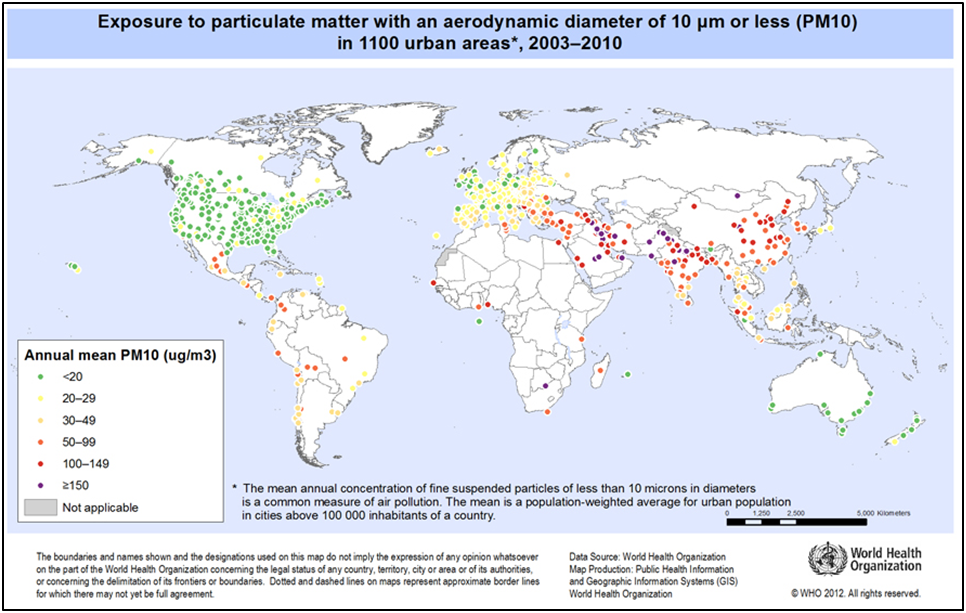
\includegraphics[scale=0.8]{images/who_pm10_world_map}
\caption{A map of \gls{pm10} in major world cities}
\label{fig:mapofpm10}
\end{figure}

As can be seen, there are many urban areas where the WHO annual mean for \gls{pm10} is exceeded. By way of example we can consider Beijing which at the time of writing (2013) had a population of 15.59m (\cite{TheUnitedNationsStatisticsDivision2013}) and was China's second largest city, is subject to seasonal dust storms, hot humid summers and cold dry winters - and suffers from severe air pollution problems. During the 1990s attempts were made at controlling air pollution in the city by introducing the use of low-sulphur coal, using natural gas as an alternative to coal, phasing out leaded petrol, and moving factories and heavy industry outside of the city. However in the early 00s, due to increasing vehicle numbers and the rapid growth of the industrial sector, particle levels continued to remain higher than national standards (\cite{Sun2004}). The nearby area of Hebei Province (which rings Beijing and is heavily industrial) made the efforts of the government to control air quality in Beijing at this time even more difficult as the Hebei region has lower fuel quality standards, and can cause some primary emissions to drift into Beijing (\cite{Tuo2013}) due to prevailing winds (Meteorology is discussed in Section \ref{subsec:meteorology}).

During the early 21$^{st}$ century the use of air pollution monitoring equipment became more commonplace and better data was collected to enable scientists to understand the issues that Beijing (and similar urban environments) faced. \cite{Sun2004} found that during the years 1999 and 2000, ambient \gls{pm25} concentrations were in the range 37 -- 357 $\mu \text{g m}^{-3}$ , and estimated a yearly average of 89.7 $\mu \text{g m}^{-3}$.  The research concluded that coal burning and traffic exhausts, along with dust from long range sources, were the major pollution sources in the urban environment of Beijing (\cite{Sun2004}).

The study of pollution in urban environments is essential as these areas are where humans are most readily exposed and they are where the sources of emissions are most frequent. Although PM has been discussed here, similar issues apply to other traffic linked pollutants such as \gls{nox} and \gls{pahs}. There are also other factors, other than the type of pollutant, that complicate the understanding of pollution in urban environments, such as weather and geography. Within these urban environments there are hyper-local conditions that can raise and lower levels. These notions are explored in sections \ref{subsec:meteorology}, \ref{subsec:urbantopography}, \ref{subsec:microenvironments} and \ref{subsec:trafficpollution}.

%%%%%%%%%%%%%%%%%%%%%%%%%%%%%%%%%%%
%%% Meteorology
%%%%%%%%%%%%%%%%%%%%%%%%%%%%%%%%%%%

\subsection{Meteorology}
\label{subsec:meteorology}

Local weather conditions have a strong influence on air quality.
%%%RAIN
Air pollution can be removed from the air in the process of cloud formation, and then deposited on the ground when the clouds turn to rain at a future time and/or place. Falling rain can also remove pollutants from the air by collecting the pollution and 'cleaning' the air as it falls. Both of these processes are grouped into the term 'wet deposition'. A 6 $\mu \text{g m}^{-3}$ difference in \gls{pm10} was observed in Edinburgh between days with no rainfall compared to those with more than 20mm of rain (\cite{DEFRA2007}). In December 2013 it was even reported that China was considering using 'cloud seeding', i.e. the process of engineering the weather to rain, as a method to lower air pollution in the most polluted regions of China (\cite{Slezak2013}).

%%%WIND DISPERSION & DILUTION
Wind can adversely affect air quality by trapping or recirculating pollutants (discussed in Section \ref{subsec:urbantopography}), but can also disperse the pollutants or move them to other areas/regions. This notion was first proposed in the 1960s when studying the acidification of lakes in Scandinavia \cite{Summers1976}, where it was theorised that the high acid levels were due to air quality elsewhere in Canada. In the UK \gls{nox} ambient concentrations were found to have halved at a monitoring station in Hillingdon, United Kingdom (\gls{uk}) when wind speed rose from 5 to 10 m/s-1, while \gls{pm25} also decreased, however the coarse \gls{pm} (\gls{pm25} to \gls{pm10}) increased due to re-suspension of particles that had previously settled (\cite{DEFRA2007}). Depending on the lifetime and properties of a pollutant, it can be transported on scales ranging from the street level to the global scale (\cite{Monks2009}). \cite{Stohl2003} found gases were being transported from North America to Europe. More locally, an odour event in the South-East of England on 18 April 2008 (\cite{TheGuardian2008}) was found to have originated from agricultural emissions in northern Germany (\cite{Smethurst2012}). The Geneva Convention on Long-range Trans-boundary Air Pollution was established in 1979 to look at ways to deal with this movement of air pollution between borders in terms of national air quality guidelines and limits, and came into force in 1983 (\cite{UnitedNationsEconomicCommissionforEurope1983}).

%%% TEMPERATURE
Direct sunlight (ultra-violet radiation) and higher temperatures, on hot summer days, can initiate reactions with nitrogen dioxide which can lead to the formation of ozone. The ozone and ozone forming chemicals remain in the atmosphere and can be transported over regional and national borders. This layer can then settle over cities such as London and lead to what is often referred to as summertime 'smog'. The South-East of England often has high concentrations during spring and summer as, amongst other sources, it is close to European pollution sources (\cite{LondonAir}). Although vehicle emissions of nitrogen oxide can have the effect of reacting with the ozone to lower the level of ozone in areas where vehicle emissions are particularly high. (\cite{EnvironmentalProtectionAgency2012}).

%%%%%%%%%%%%%%%%%%%%%%%%%%%%%%%%%%%
%%% Urban topography
%%%%%%%%%%%%%%%%%%%%%%%%%%%%%%%%%%%

\subsection{Urban topography}
\label{subsec:urbantopography}

In the urban environment, streets are often bordered by tall buildings which can influence pollution levels for people at ground level. Topography of this nature is often referred to as a 'street canyon'. In extreme circumstances such as on the streets of Hong Kong, skyscrapers are littered throughout the city, but on smaller scales such as Oxford Street (London, \gls{uk}) similar issues occur but with modest building heights. Being bordered by tall buildings creates a sheltering effect from the wind, stopping particles being moved elsewhere. The typical street-canyon effect occurs when there is a steady flow over the top of tall buildings (see figure \ref{fig:street_canyon}), where the mean flow is perpendicular to the direction of the street (\cite{Britter2003}). With roof-level wind-speeds of 1.5-2 m/s, the air is recirculated within this 'box' and air quality deteriorates as sources (usually traffic) emit more fumes.

\begin{figure}[H]
\centering
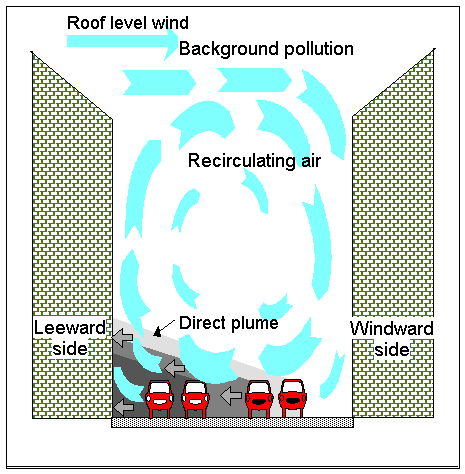
\includegraphics[scale=0.7]{street_canyon}
\caption{Pollutant dispersion in a regular street canyon}
\label{fig:street_canyon}
\end{figure}

Mexico City is an example of a city that is subject to this effect on a large scale. Situated in central Mexico, North America (19.4328° N, 99.1333° W), Mexico City is one of the most populated cities in the world and has an estimated population of about 21m (2011) living within the Mexico City Metropolitan Area (MCMA) of 1,485 km\textsuperscript{2} (\cite{TheUnitedNationsStatisticsDivision2013}). Mexico City is located in the crater of a large extinct volcano, which means that the entire city suffers from the aforementioned canyon effect. Almost like it is surrounded by skyscrapers. This is exacerbated by a fleet of older vehicles with poor engines (the effects of which are discussed more in Section \ref{subsec:trafficpollution}), low levels of oxygen (due to the high altitude of the city), and wind patterns that concentrate pollutants in the western and southern parts of the city (\cite{Garza1996}) where the population is most dense.

To summarise, air pollution in the urban environment can be effected by the meteorology and topography of the area. On the smaller scale than 'area' there are also micro-environments that people spend time in, for example inside a bus, which can exhibit very different characteristics than the rest of the city or even street.

%%%%%%%%%%%%%%%%%%%%%%%%%%%%%%%%%%%
%%% Micro-environments
%%%%%%%%%%%%%%%%%%%%%%%%%%%%%%%%%%%

\subsection{Micro-environments}
\label{subsec:microenvironments}
Micro-environments are defined as the immediate small-scale environment of an organism, especially as a distinct part of a larger environment. Examples in the context of this thesis include the air quality inside a vehicle, a house or  underground train carriage, in the context of the environment outside. Understanding how pollutant levels change in these micro-environments is key, as much of our time is spent within these environments, thus our exposure level to air pollutants whilst in them could have important impacts on our health.

%%%%%%%%%%%%%%%%%%%%%%%%%%%%%%%%%%%
%%% Indoors
%%%%%%%%%%%%%%%%%%%%%%%%%%%%%%%%%%%
\subsubsection{Indoors}
\label{subsubsec:indoors}

The most common micro-environment is within buildings, the air we are exposed to when we are at home, in the office or at school etc. WHO calculated in 2005 that people spend 89\% of their time indoors (\cite{WorldHealthOrganization2005}). In these environments, people are exposed to pollutants generated outdoors that penetrate to the indoor environment, as well as to pollutants produced indoors. The EXPOLIS study \cite{Kousa2002} examined how much time people spend in these environments by asking 1427 people from accross Europe (Athens (Greece), Basle (Switzerland), Grenoble (France), Helsinki (Finland), Milan (Italy). Oxford (Great Britain) and Prague (Czech)) to complete activity diaries. They found that the amount of time people spend indoors varied by whether the people were employed or not, in what type of job, whether they lived alone and/or whether they had children. Gender and season of year were also found to be factors. Study participants were found to spend on average 13.95 hours indoors at home (13.48 min to 15.76 max) and 6.71 hours indoors at work (5.09 to 7.09) (\cite{Schweizer2007}). So understanding indoor air quality, which would include filtration of outdoor air into the building as well as pollutants whose sources are inside, is important in understanding personal exposure. However research on indoor pollution has not had the same focus as outdoor pollution for a number of reasons. Firstly the perceived need to deal with coal and traffic emissions, the ease of monitoring outdoor air quality using fixed monitoring sites (compared to monitoring every home). Secondly epidemiologists have traditionally only linked outdoor ambient pollutant concentrations to health health issues, furthermore, legislating the air that people can breathe in their own homes can be seen as intrusive to people's private lives, finally  the funding and policy initiatives around air pollution research has mainly come from developed countries, which who do not have such an issue with indoor pollution as low and middle income countries (\cite{WorldHealthOrganization2010}) (due to low and middle income countries using solid fuel for cooking and heating inside their homes more).

The pollutants that are emitted indoors, and which the US Environmental Protection Agency (\gls{usepa}) focus on in their guide to indoor air pollution, include Volatile Organic Compounds (\gls{vocs}), \gls{co} and \gls{no2} (\cite{UnitedStatesEnvironmentalProtectionAgency2008}). \gls{vocs} in indoor air come mostly from products used around the house such as paint, varnish, cleaning sprays, air fresheners and pesticides but can also be emitted by building materials and furnishings. \gls{co} and \gls{no2} on the other hand are more commonly associated with the use of indoor furnaces, gas cookers, gas heaters, leaking chimneys and people smoking tobacco indoors.

The \gls{usepa} report however, only focuses on indoor air pollution relevant to buildings in the United States (US). In different parts of the world indoor air quality varies in terms of the pollutants and the impact, especially in Asian countries where less clean combustion fuels are often used for cooking in the home and the numbers of people that smoke while indoors is greater (\cite{Lee2010}). 
\cite{Baumgartner2011} sampled \gls{pm25} in 44 kitchens of the Yunnan area of China in 2010, where 95\% of the kitchens used wood or crop residue for cooking, and 96\% used a mix of wood-charcoal and wood or crop reside for heating. During the summer months, when the sampling was done, mean concentrations were found to be around 107 $\mu \text{g m}^{-3}$. Similarly, \cite{Li2011} compared pollutant concentrations in kitchens in relation to different types of stoves in Peru. Means of 181 $\mu \text{g m}^{-3}$ and 3.5 ppm were found for the open-pit stoves for \gls{pm25} and CO respectively. In a larger study across 168 venues in China, Japan, Korea, Malaysia, Pakistan and Sri-Lanka, \gls{pm25} measurements were made and an average indoor level of 137 $\mu \text{g m}^{-3}$ was found (smoking venues were 156 $\mu \text{g m}^{-3}$, non-smoking venues were 34 $\mu \text{g m}^{-3}$).

Poor indoor air quality is not always due to indoor sources. The pollutant levels outside an indoor environment have been found to have an impact, although this is dependant on many mitigating factors such as the buildings air filtration units, proximity to outdoor sources, and wind speed/direction. In North America, homes close to Ambassador Bridge (Detroit) were measured over five 24 hour periods \cite{Baxter2008} and it was found that ambient black carbon concentrations significantly contributed to indoor concentrations regardless of wind speed. In Osaka, Japan fine \gls{pm} (\gls{pm25}) was significantly correlated with fine \gls{pm} outside the properties and it was estimated that about 30\% of indoor \gls{pm10} particles were from diesel exhausts from nearby roads (\cite{Funasaka2000}). In Europe (Prague, Czech Republic) \gls{pm25} was sampled in a school gym during 2005 and 2006, and levels were found to be similar to a nearby fixed-site monitor (24.03 $\mu \text{g m}^{-3}$ compared to 25.47 $\mu \text{g m}^{-3}$) (\cite{Branis2009}).

%%%%%%%%%%%%%%%%%%%%%%%%%%%%%%%%%%%
%%% In-vehicle
%%%%%%%%%%%%%%%%%%%%%%%%%%%%%%%%%%%
\subsubsection{In-vehicles}
\label{subsubsec:invehicle}

The air quality people are exposed to when travelling between indoor micro-environments i.e. a bus or train or car, can differ greatly from general ambient concentrations. Similarly, when space inside vehicles has its own air quality micro-environment. Conditions can be affected by having windows open or closed, the type of vehicle, and the vehicle's location amongst other factors. \cite{Adams2001} measured \gls{pm25} during 465 journeys in London over a three week period, at peak and off-peak times of the day during the summer of 1999 and winter of 2000.

\begin{table}[H]
\caption{\gls{pm25} by transport mode}
\centering
    \begin{tabular}{ | l | l |}
    \hline 
     \bfseries{Transport mode} & \bfseries{Mean ($\mu \text{g m}^{-3}$)} \\ \hline
     Bus & 39.0\\ \hline
     Car & 37.7\\ \hline
     Underground tube & 247.2\\ \hline
     Overground tube & 29.3\\ \hline
    \end{tabular}
\label{tab:adams_transport_means}
\end{table}

They observed a great deal of variability between travel modes (see table \ref{tab:adams_transport_means}), and against typical ambient \gls{pm25} levels (around 10-30 $\mu \text{g m}^{-3}$) recorded for central London. Outside of London, also in 1999/2000, \cite{Gulliver2004} conducted in-vehicle monitoring along a stretch of road in Northampton (80 km North/North West of London). They also observed elevated levels of particulates inside the vehicle (table \ref{tab:gulliver_vehicle_means}).

\begin{table}[H]
\caption{In-vehicle \gls{pm}}
\centering
    \begin{tabular}{ | l | l |}
    \hline 
     \bfseries{\gls{pm} Fraction} & \bfseries{Mean ($\mu \text{g m}^{-3}$)} \\ \hline
     \gls{pm10} & 43.16\\ \hline
     \gls{pm25} & 15.54\\ \hline
    \end{tabular}
\label{tab:gulliver_vehicle_means}
\end{table}

Neither of these authors comment on air quality inside vehicles or the resultant exposure. They only conclude that in-vehicle pollutant concentrations cannot be taken to be the same as outdoor values. The situation is further complicated by additional variables such as whether windows are open or closed, the speed of the vehicle, or the number of people inside the vehicle.

%%%%%%%%%%%%%%%%%%%%%%%%%%%%%%%%%%%
%%% TRAFFIC POLLUTION
%%%%%%%%%%%%%%%%%%%%%%%%%%%%%%%%%%%

\subsection{Traffic pollution}
\label{subsec:trafficpollution}

%%% THE NUMBERS OF VEHICLES HAS CHANGED DEPENDING ON WHERE IN THE WORLD YOU LOOK
Between the years of 1950 and 1994, there was a dramatic increase in vehicle traffic on the worlds roads. Vehicle numbers increased from 53 million, to 460 million in the space of 44 years (\cite{TheWorldBank2013}). Against this backdrop of increasing numbers of vehicles, there is emerging evidence that traffic emissions are harmful to human health. In 2010 the US Health Effects Institute (\gls{ushei}) published the findings of a systematic review of evidence about traffic pollution, and whilst noting that there were many areas still needing further research, there was evidence to support a casual relationship between exposure to traffic-related air pollution and asthma (\cite{HPotHEoT-RA2010}). Toxicological research has now also started to link not only primary traffic emissions i.e. exhaust, but also non-exhaust pollutants such as road abrasion, tyre wear and brake wear to adverse health effects (\cite{WorldHealthOrganization2013}). The latter being particularly significant given that there are no laws which consider this element of traffic pollution and therefore no guidelines or limit values. Despite this, measuring and characterising emissions that are solely solely attributable to traffic sources in the urban environment is technically difficult, which makes linkages with exposure estimates and health effects problematic. Different studies have therefore used different pollutant concentrations as markers for traffic emissions. Epidemiological studies have often used \gls{no2} as a marker for combustion-related pollutants, in particular those emitted by road traffic or indoor combustion sources (\cite{WorldHealthOrganization2010}).

%%% LET'S LOOK AT BEIJING AS A CASE STUDY AND SEE A BIT MORE ABOUT TRAFFIC POLLUTION
Taking the city of Beijing as example again, in 2008 the Olympic Games were held there and this heightened the world’s interest in Beijing's air quality and put the issue under national scrutiny. Global newspapers focused on the effects that poor air quality might have on the performance of the athletes. The reporter James Reynolds of the British Broadcasting Corporation (\gls{bbc}) wrote "\textit{China is spending billions of pounds on new roads, new venues and on perfect celebratory shows but all that may come to nothing unless this city cleans up its air}" (\cite{BBC2007}). Under this pressure, to try and bring air quality problems under control (at least in the short term while the Olympics were taking place) the Beijing Government implemented a number of measures in the run-up to the games. Stricter vehicle emission standards were adopted, better public transport infrastructure was developed, and from July 2008 to September 2008 a traffic demand management scheme was introduced whereby odd/even vehicle registrations took it in turns to be used on the roads on alternate days (\cite{Wang2009}). This provided an ideal real-world experiment for the local scientists to attempt to quantify how much poor air quality in the city was attributable to vehicle emissions. Data on black carbon levels was collected by fixed background and fixed road-side monitors, and then analysed to investigate whether the scheme had achieved the desired effect.

\begin{figure}[H]
\centering
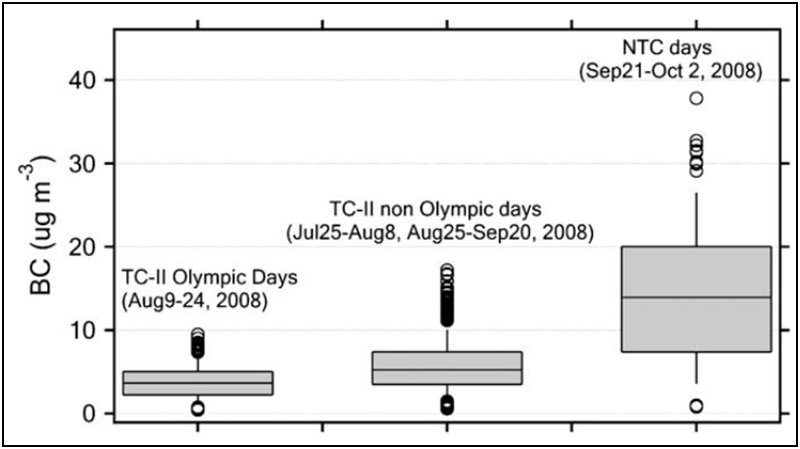
\includegraphics[scale=1]{black_carbon_olympic}
\caption{Black carbon concentrations during 2008 in Beijing}
\label{fig:blackcarbonolympic}
\end{figure}

The results from this study are shown in figure \ref{fig:blackcarbonolympic} and demonstrate how mean black carbon concentrations dropped to around 5 $\mu \text{g m}^{-3}$ during the Olympics (second boxplot) compared to around 14 $\mu \text{g m}^{-3}$ after the Olympics (third boxplot). In addition, during the Olympics on days when the main sporting events were happening, there was a further reduction to around 4 $\mu \text{g m}^{-3}$ (first boxplot). The traffic in Beijing, at least within the limits of this small subset of data, seemed to be contributing to around 10 $\mu \text{g m}^{-3}$ of black carbon pollution in the air. The authors of this study go on to conclude that the main source of emissions in Beijing at the time are from traffic, and that the traffic demand management scheme was effective at bringing emissions down to the (\gls{who}) objective levels. However this seems to be a simplification of the issue, especially given the impact of factories in the vicinity (discussed in \ref{subsec:urbanenvironments}). Nonetheless, the exposure of the residents of Beijing to pollution, a debatable proportion of which is from tailpipe emissions, is high.

%% Now lets look at a more Western city

In Europe, where factories and heavy industry tend not to be based within urban centres, the proportion of the population's exposure to poor air quality, originating from traffic, is high. Often, due to meteorology (see \ref{subsec:meteorology}), some emissions may also be from other urban centres. For example emissions from outside London are estimated to account for around 40\% of \gls{no2} concentrations (with the other 60\% being generated locally) (\cite{GreaterLondonAuthorityGLA2010}. This ratio changes depending on different spatial resolutions. In areas close to roads, the contribution of traffic emissions to overall air quality levels is much higher due to the proximity to the sources (vehicles). The influence of traffic emissions on ambient concentrations is well demonstrated by \cite{Mayer1999}. Figure \ref{fig:stuttgarttraffic} identifies clear trends related to rises in \gls{no} and \gls{no2} during morning and evening rush hours on working days.

\begin{figure}[H]
\centering
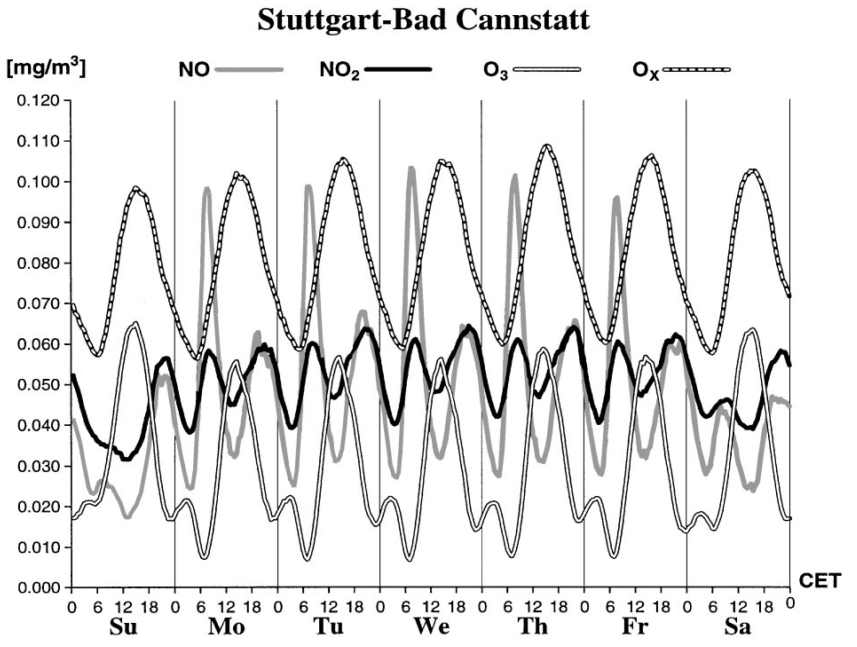
\includegraphics[scale=0.6]{stuttgarttraffic}
\caption{Average weekly and diurnal cycles of \gls{no}, \gls{no2} ,\gls{o3} and \gls{nox} at the urban air-quality station Stuttgart-Bad Cannstatta for the period 1981-1993}
\label{fig:stuttgarttraffic}
\end{figure}

%% What's going on with policy attempts to reduce.
 
As air pollution from vehicles is harmful to health, and traffic pollution is so prevalent in urban environments, more permanent long-term attempts to reduce traffic pollution are ongoing in most major cities and countries around the world. Though different countries have sought to achieve this in different ways. An article on 'The Conservation' website \cite{Williams2013}) explains how the \gls{eu} attempted to legislate to reduce vehicle emissions (\cite{Williams2013}), prompted by the Kyoto Protocol of 1997 which was linked to the United Nations Framework Convention on Climate Change (\cite{UnitedNations1998}). The protocol sought to specifically reduce CO$_{2}$ emissions by a) legislating that car retailers must provide buyers with information on vehicles' fuel consumption and \gls{co2} emissions and b) placing limits on \gls{co2} emissions, as a ratio of kilometres travelled, to encourage more efficient use of fuel and therefore lower emissions. The legislation also encouraged companies making vehicles for the EU markets to invest in the production and marketing of diesel vehicles, as they were more fuel efficient than petrol vehicles. In conjunction, these measures were designed to encourage a change in manufacturers behaviour leading to lower emissions through a 'free-market' approach. Unfortunately it became apparent that diesel cars emit higher levels of emissions than petrol cars fitted with three-way catalytic converters (\cite{Williams2013}). The difference between the two emission levels are even greater when considered in the real-world rather than measured in laboratory conditions (\cite{Carslaw2011}). A study in 2007 estimated that the health effect of favouring diesel vehicles over petrol vehicles in the UK has had the combined effect of contributing to approximately 1850 additional premature deaths over the period 2001-2020, or around 90 premature deaths per year (\cite{Mazzi2007}).

%% The alternative is different vehicles altogether.
There are of course vehicles that produce low or even zero emissions i.e. hybrid or electric. Hybrid vehicles use a mixture of fuel (petrol or diesel) and a battery, and electric vehicles run solely from a battery.  Unfortunately for air quality in urban environments these types of vehicle are currently only a very small percentage of new vehicles, for example in the third quarter of 2018 only 2.2\% of new vehicle registrations in London were low or zero emission (\cite{TFL2018}).

%%%%%%%%%%%%%%%%%%%%%%%%%%%%%%%%%%%
%%% Summary of what is air pollution
%%%%%%%%%%%%%%%%%%%%%%%%%%%%%%%%%%%
\subsection{Summary}
\label{subsec:whatissummary}

Section \ref{sec:whatisairpollution} introduced the subject of air pollution -- a non-naturally occurring material in the air, altering it's composition. It can take many different forms and be categorised in different ways, for example particulate matter, nitrogen oxides, ozone or sulphur dioxide. It was discussed how many of the causes of air pollution are linked to vehicle combustion engines and that in urban environments, where people are increasingly living, this places the sources and public in close proximity to each other. This can be affected (both positively and negatively) by different meteorological conditions and the topology of the region, city, and even individual streets and buildings. Within these environments, it was explained that there are micro-environments such as inside vehicles and buildings which can also raise or lower pollution levels. As this research intends to focus on urban environments, traffic emissions were then considered in a little more detail. The Beijing Olympics 2008 was used as a case-study to understand the impact that traffic emissions can have on air quality in a major city, and the diesel dominated vehicle fleet of Europe was then explained (touching on the impact compared to petrol that this has had on air quality).

Now that the subject of air pollution has been introduced, the next section of this background will give an overview of the impact on human health from air pollution i.e. why Section \ref{sec:whatisairpollution} actually matters to us.

\newpage
%%%%%%%%%%%%%%%%%%%%%%%%%%%%%%%%%%%%%%%%%%%%%%%%
%%% AIR POLLUTION AND HEALTH SECTION %%%%%%%%%%%
%%%%%%%%%%%%%%%%%%%%%%%%%%%%%%%%%%%%%%%%%%%%%%%%
\section{Health effects of air pollution}
\label{sec:healtheffects}

\begin{quote}
"Clean air is considered to be a basic requirement of human health and well-being. However, air pollution continues to pose a significant threat to health worldwide" (\cite{WorldHealthOrganisation2006}).
\end{quote}

\subsection{An overview}
\label{subsec:anoverview}

%%%%%%%%%%%%%%%%%% Where concerns about air pollution and health came from

%https://www.hsph.harvard.edu/news/press-releases/air-pollution-premature-death-u-s-seniors/
%“We found that the mortality rate increases almost linearly as air pollution increases. Any level of air pollution, no matter how low, is harmful to human health.”

From the 1600’s onwards coal was the main source of heat and energy in major \gls{uk} cities. Concern from the scientific community and coherent programs of research about the possible negative effects of this fuel source were limited. When undertaken the research often focused on poor visibility or damage to buildings rather than human health. It was the early 1900’s when coherent and robust studies began to investigate mortality and links to ‘fog’, as it was known at the time. Notably with Russell’s paper \textit{'The Influence of fog on mortality from respiratory diseases'} being published in The Lancet in 1926 (\cite{Russell1926}). This publication preceded London's 'Great Smog' of 1952, which was one of the \gls{uk}'s most important air pollution events in history in terms of realisation of the links between pollution and health. Research conducted since this event has had a great impact on the study of air pollution, public perception and government regulation to combat it. Data at the time showed that a rise in fog (pollution) levels was closely followed by rises in mortality and morbidity (\cite{Bell2003}). At the time it was estimated that between 3,500 and 4,000 more people died than would have normally been the case in this period (See figure \ref{fig:greatsmogdeaths} from \cite{GreaterLondonAuthorityGLA2002}). The rise in mortality was originally attributed to influenza, however sensitivity analysis by \cite{Bell2003} revealed that only an extremely severe influenza epidemic could have accounted for the excessive deaths recorded for that period. Subsequent reanalysis of the data estimated that between December 1952 and March 1953 there were actually 13,500 more deaths than during the same time period the previous year, attributable to (controlling for temperature and influenza) rather than the 3000--–4000 generally reported for the episode.

\begin{figure}[H]
\centering
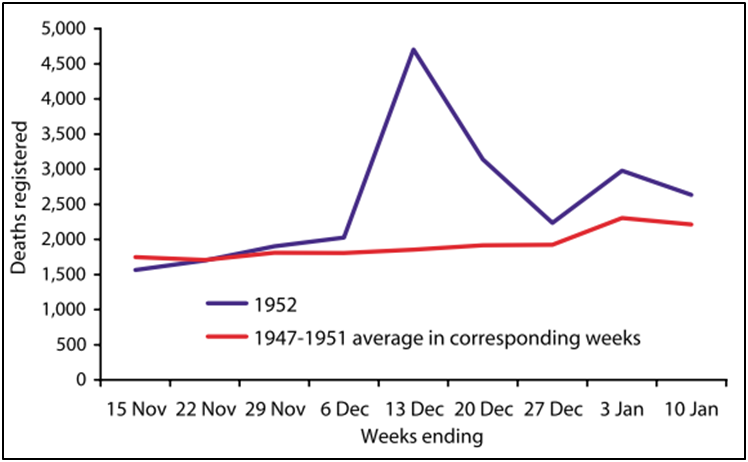
\includegraphics[scale=1.2]{great_smog_deaths}
\caption{Recorded deaths comparison during 'Great smog' period. 1952 (blue line) shows a peak in deaths coinciding with the 'great smog' which is not seen in the preceding or following years (red lines)}
\label{fig:greatsmogdeaths}
\end{figure}

%%%%%%%%%%%%%%%%%% Some laws and EU regs were passed over time

Once this explicit link between air pollution and health became apparent, laws and regulations began to be written and passed. For example the Clean Air Act in 1956 (with various revisions over time, notably in 1968), the 1970 European Commission (\gls{ec}) Directive (70/220/EEC), the 1974 Control of Pollution Act and the 1979 International Convention on Long Range Transboundary Pollution.
%%%%%%%%%%%%%%%%%% Now widely accepted that it's harmful to health
It is now widely accepted that air pollution has harmful effects on human health (\cite{WorldHealthOrganization2013}. Although in the Western world, the sources of pollution have shifted from using coal for heating and cooking, to be dominated by combustion engines in vehicles and similar (as discussed in Section \ref{subsec:trafficpollution}).


%%%%%%%%%%%%%%%%%% Epidemiology is _______. Looks at risk factors between exposure and health effects. Allows large scale effects to be examined across populations. Although it can be confusing in the variation, 
When considering the effects of air pollution on public health, studies on large groups of people (tens of thousands plus) often use epidemiological methods. Studies using epidemiological methods will be discussed many times during this thesis, therefore a brief definition of epidemiology and the key terms are now given.

Epidemiology is the the study of how often disease/poor health occurs in a group of people, and the factors that lead to it. Or, more technically defined by Bonita in a \gls{who} publication as \textit{'the study of the distribution and determinants of health-related states or events in specified populations, and the application of this study to the prevention and control of health problems'} (\cite{Bonita2006}). Some key terms include (adapted from \cite{U.S.DepartmentofHealth&HumanServices2014}):

\begin{itemize}
\item Incidence: The number of new ill people in the population over a specified time period
\item Prevalence: The existing number of ill people in the population over a specified time period.
\item Burden of disease: The total significance of the disease or illness to wider society. For mortality this is often measured in years of life lost.
\item \gls{daly} (Disability-Adjusted Life Year): A statistic to represent the health of a population. One DALY represents one lost year of healthy life and is used to estimate the gap between the current health of a population and an ideal situation in which everyone in that population would live into old age in full health.
\end{itemize}

%%%%%%%%%%%%%%%%%% Using epidemiology-like studies, health issues from air pollution include x, y, z. Also recently IARC cancer stuff.
Epidemiological studies have '\textit{For decades [ ... ] been a cornerstone of our approach to investigating the health effects of air pollution and have been a principal basis for setting regulations to protect the public against adverse health effects}' \cite{Zeger2000}. Recent high profile examples that look at air pollution include, but are not limited to; respiratory problems (\cite{Peacock2011}), cardiovascular issues (\cite{Brook2010}) and cancer (\cite{Iii2012}, \cite{loomis2013}). Indeed, recently (17 October 2013), the International Agency for Research on Cancer (\gls{iarc}) classified outdoor air pollution as carcinogenic to humans (\cite{loomis2013}). In an \gls{iarc} press-release, Dr Kurt Straif, Head of the Monographs Section stated \textit{"The air we breathe has become polluted with a mixture of cancer-causing substances. We now know that outdoor air pollution is not only a major risk to health in general, but also a leading environmental cause of cancer deaths"}.

%%%%%%%%%%%%%%%%%% The strongest association found thus far is between poor health and PM2.5

However as discussed in Section \ref{subsec:particletypesandsizes}, the term 'air pollution' covers many different pollutants. It is important therefore to untangle which pollutants are more or less harmful to health. This will help people avoid areas with pollution that is most harmful, and help politicians to develop policies that are effective at reducing the most harmful types of pollution. For example there is good evidence that the \gls{pm25} shortens life, however it tends to be emitted in locations where there are sources of other pollutants such as \gls{no2}, which makes it hard to disentangle the effects of them individually (\cite{CommitteeontheMedicalEffectsofAirPollutants2018}). A broad overview of epidemiological studies on the health effects of exposure to \gls{pm25} is now discussed.

%%%%%%%%%%%%%%%%%% Across the world it causes X premature deaths
Worldwide, WHO estimate that \gls{pm25} causes about 9\% of lung cancer deaths, 5\% of cardiopulmonary deaths, and 1\% of respiratory infection deaths (\cite{WorldHealthOrganization2012}). In 2013 the Global Burden of Disease publication ranked exposure to air pollution and particulate matter as one of the top ten risk factors for health globally, estimating that over 430,000 premature deaths and around 7 million years of healthy life were lost in Western, Central and Eastern Europe in 2010 from exposure to fine particulate matter (\cite{Brauer2012}) n.b. fine refers to particulate matter smaller than 1 micron in diameter, ultrafine smaller than 2.5 microns (includes the 1 micron particles), and coarse smaller than 10 microns (includes the 1 and 2.5 micron particles). 

In a study looking at \gls{pm25} and anthropogenic ozone, \cite{Silva2013} recently modelled ozone and \gls{pm25} surface concentrations for the entire world, then used concentration-response functions for long-term exposure and mortality (from an American Cancer Society publication) to estimate that annually and globally there are about 2.1 million premature deaths from respiratory problems linked to \gls{pm25}, with these being split 93:7 between cardiopulmonary disease and lung cancer (\cite{Silva2013}).

We can therefore see that the health effects of \gls{pm25}, when taken in context of large populations are significant. However, these figures are likely to be the tip of a much larger concern as most do not include morbidity i.e. poor health and detriments to the populations quality of life that do not result in death. This is illustrated by figure \ref{fig:airpollutionpyramid} (\cite{Mannino2000}) showing a greater number of the population have less severe health effects that still have a burden on public well-being.

\begin{figure}[H]
\centering
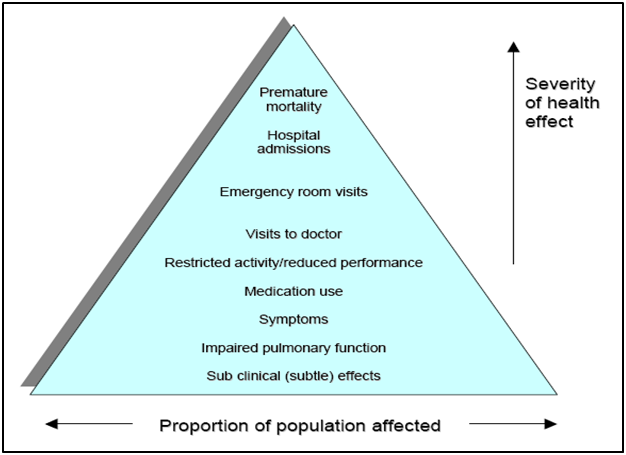
\includegraphics[scale=1.4]{air_pollution_pyramid}
\caption{Air pollution health effects pyramid}
\label{fig:airpollutionpyramid}
\end{figure}

%%%%%%%%%%%%%%%%%% In the UK we have COMEAP. Some estimations on air pollution/health impact are mentioned.

In the \gls{uk}, the Committee on Medical Effects of Air Pollutants (\gls{comeap}) has been set-up to provide advice to the government and related agencies via the Department of Health's Chief Medical Officer on the harmful effects of air pollution. COMEAP regularly publish reports summarising findings into the health effects of pollutants. In their 2010 report on mortality, they estimated that around 29,000 deaths in the \gls{uk} in 2008 were attributable to \gls{pm25} (\cite{CommitteeontheMedicalEffectsofAirPollutants2009}). Expressing this differently, they estimated that air pollution may have contributed to the earlier deaths of about 200,000 people in 2008, with an average loss of life of about two years per death affected. Also on a \gls{uk} scale, \cite{Yim2012} estimated that \gls{pm25} causes about 19,000 premature deaths in the \gls{uk} and 3,200 in London. Note that the reason for these figures being lower than that of \gls{comeap} is that this study focused solely on the deaths attributable to traffic emissions rather than all sources (and gives at least in this context a rough idea of the impact of traffic emissions compared to non-traffic emissions). At the city level, \cite{Miller2010} used life-tables and concentration-response coefficients to estimate deaths attributable to \gls{pm25} to be 4,267 in Greater London for 2008.

%%%%%%%%%%%%%%%%%% But how does it actually cause these effects? Epi gives us broad stuff. What’s actually happening?

While epidemiological studies find strong links between air pollution and poor health, particularly pulmonary and cardiovascular disease, the mechanism of \textbf{how} air pollution causes mortality is not yet fully understood. 

%%%%%%%%%%%%%%%%%% People have tried to identify the specific pathways and effects using chambers studies too. These are useful as they can identify specific pollutants rather than in the atmosphere where they are mixed.

Chamber studies are often used to identify the toxicological effects of air pollutants. Human subjects will be medically examined before entry to the chamber, then sealed inside for a set period of time, and re-examined after exposure to pollutants. The atmosphere within can be carefully controlled by investigators to simulate the environment of their choice, in the case of air pollution normally this is heavily polluted air. Lung function tests, haematology and fiberoptic bronchoscopy are undertaken to investigate the pathological pathways by which pollutants may cause disease and poor health.

\cite{Salvi1999} exposed 15 healthy human volunteers in an environmental chamber to  clean air and then diluted diesel exhaust, for one hour at a time. Significant increases in neutrophils and platelets, markers of stressed airways and lungs, were observed in the subjects peripheral blood after the diesel exposure, however lung function measured before and after exposure revealed no decline. The study demonstrated that at high concentrations of diesel exhaust, at least in the short term, there is a systemic and pulmonary inflammatory response in healthy human volunteers, which is not detected by standard lung function measurements alone. A further study by \cite{Salvi2000} exposed healthy human volunteers in chambers to a range of particles/diesel exhaust and fiberoptic bronchoscopy was performed six hours after each exposure, the results suggest airway leukocyte infiltration as the underlying mechanism for diesel exhaust-induced respiratory health outcomes. In a study by \cite{Ghio2000} no immediate symptoms were observed, however 18 hours after exposure inflammation was identified in the lower respiratory tract, particularly in those with the highest particulate exposure compared to clean filtered air.

The afore-mentioned studies suggest that pulmonary inflammation in the airways is responsible for damage to the lungs. Although more studies are needed to pin-point the specific pathways. Chamber studies have helped to understand the inflammation pathways following short-term, however further issues also need to be addressed, for example, the lack of clarity between the length of exposures and the subsequent responses and how long the lag is between exposure and underlying biological mechanism responses (such as in the studies just mentioned where different effects were noted after 6 hour and 18 hours) (\cite{EnvironmentalProtectionAgency2009}).

To summarise, the American Heart Association (AHA) \cite{Brook2010} describe the probable mechanism between particulate matter air pollution and cardiovascular disease as the following:

\begin{enumerate}
  \item Release of proinflammatory mediators (eg, cytokines) from activated immune cells, or platelets or vasculoactive molecules (eg, Endothelin, histamine), or microparticles endothelium of blood vessels in the lung
  \item Perturbation of systemic autonomic nervous system balance or heart rhythm by particle interactions with lung receptors or nerves
  \item Translocation of PM (ie, ultrafine particles) or particle constituents (organic compounds, metals) into the systemic circulation
\end{enumerate}

%%%%%%%%%%%%%%%%%% It's not fully understood. But here are some ideas and possible mechanisms.

A simplified diagram from the same reference (\cite{Brook2010}) has been adapted and is shown below (fig \ref{fig:biological_pathways}) for illustrative purposes.

\begin{figure}[H]
\centering
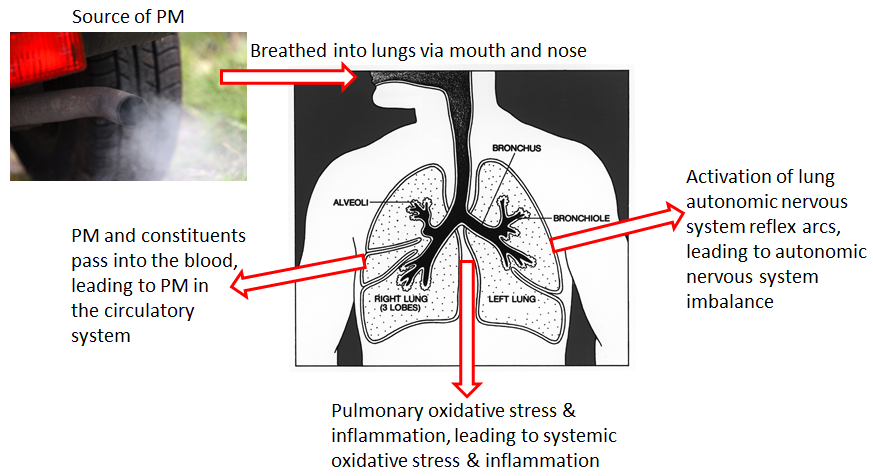
\includegraphics[scale=0.6]{biological_pathways}
\caption{The biological pathways linking PM exposure with cardio--vascular disease}
\label{fig:biological_pathways}
\end{figure}

%%%%%%%%%%%%%%%%%% However I’m not going to dwell on specific pathways and biology. Suffice to say there’s something going on. Maybe it’s short term. Maybe it’s long term. Maybe it’s a combination of the both (seems most likely). But the ways of looking into it are varied.

A detailed review of the biological mechanisms underlying disease is not the scope of this thesis. Rather it is concerned with the methods of estimating levels of exposure to air pollution. The presumption of this research is that even low levels of exposure to air pollution is harmful. This is justified by studies such as the European ESCAPE project (\cite{Beelen2013}) which found that long-term exposure to fine particulate pollution is associated with mortality, even at concentration ranges well below the present European annual mean limit values. The work of \cite{Brauer2002} and his group looked at the use of minimum threshold values for exposure to \gls{pm25} and found that due to exposure miss-classification, population-level thresholds were apparent at lower ambient concentrations than common personal thresholds (such as the EU limit values discussed in table \ref{tab:whopmlevels} of Section \ref{subsec:urbanenvironments}).

In summary, epidemiological and toxicological studies have shown air pollution is a major environmental risk to health. By reducing air pollution levels, and exposure to air pollution, governments should be able to reduce respiratory symptoms, heart disease, and lung cancer in their population. In order to calculate the estimates of the detrimental effects on people's health, exposure and dose must be calculated as accurately as possible. That is the amount and types of air pollution that people are exposed to, and breathe in,every day of their lifetime. This can be done in many different ways, and methods are undergoing regular revision as scientists attempt to improve their accuracy. 

One of the key issues to address to further understand the links between pollutant exposure and poor health is the duration of exposure. Does long-term exposure to low levels of pollution have the same effect as short-term exposure to high levels of pollution in terms of disease prevalence or \gls{daly} The importance of short-term versus long-term exposure on health is explored in the next section.

%%%%%%%%%%%%%%%%%%%%%%%%%%%%%%%%%%
%%% Long term v short term
%%%%%%%%%%%%%%%%%%%%%%%%%%%%%%%%%%

\subsection{Long term exposure v. short term exposure}
\label{subsec:longtermvshortterm}

%%%%%%%%%
There are few studies that compare the effects of long and short-term exposure to air pollution on a large population, at adequate spatial and temporal scales, for a range of pollutants, and with appropriate health information to enable us to determine which has the most impact on health.

%The approach that investigators have used when attributing exposure and dose values to groups of subjects for health studies (and the limitations thereof) are discussed more in sections \ref{sec:staticexposurehealth} and \ref{sec:dynamicexposurehealth}, and indeed form a crucial aspect of this research, however methods of exposure  aside, which of short-term or long-term exposure to air pollution is a more important contributor to poor health is not yet properly understood and is an issue that is being wrestled with by the community at present. 

This section therefore presents a selection of the short term and long term studies conducted to date, as well as the small number of studies that have attempted to reconcile the two. This is an issue that is being wrestled with by the community at present.

The most widely cited large-scale long-term exposure/health studies are on the effects of \gls{no2} in New Zealand \cite{Scoggins2004}, fine particles globally in the Global Burden of Disease 2010 ( \cite{Brauer2012}) and a meta-analysis review of both by \cite{Faustini2014}. Scoggins modelled annual average \gls{no2} concentrations over 3 km x 3 km grid squares in Auckland for the years 1996-1999 and linked these to mortality data for the same region provided by the Health Information Service (estimating a 1.3\% increase in mortality for each 1 $\mu \text{g m}^{-3}$ rise in \gls{no2} annual average values), Brauer used global estimates of ozone and \gls{pm25} concentrations at a 0.1\textsuperscript{o} x 0.1\textsuperscript{o} spatial resolution  to inform the global burden of disease modelling (discussed previously in Section \ref{subsec:anoverview}), and Faustini's review brought together studies that looked at \gls{no2} and \gls{pm25} on population mortality and found that there was rise of 1.04\% and 1.05\% per years of life per 10 $\mu \text{g m}^{-3}$ for \gls{no2} and \gls{pm25}, respectively. Meta-analysis by \cite{Hoek2013} estimates an excess risk of 6\% per 10 $\mu \text{g m}^{-3}$ increase in \gls{pm25} exposure.

As stated, links between long-term exposure and poor health seem to be fairly robust, however as long exposure time-frames that are used (typically annual average concentrations), and are combined with large spatial scales of hundreds of kilometres, it is possible that much of the detail in the results is being missed - which will be discussed more in sections \ref{sec:staticexposurehealth} and \ref{sec:dynamicexposurehealth}. Furthermore, no short-term exposure on health effect outcomes from poor air quality are considered in these 'long-term' studies, or a comparison of the importance of long-term versus short-term exposure effects.

On the flip-side, short-term epidemiological exposure health studies tend to suffer from similar issues from the perspective of someone trying to weigh-up short-term versus long-term exposure. The review by \cite{Brook2010} (briefly discussed earlier in \ref{subsec:anoverview}) concluded that short-term epidemiological time-series studies tend to find that around a 10 $\mu \text{g m}^{-3}$ increase in mean 24-hour \gls{pm25} concentrations increases the risk of cardiovascular mortality by approximately 0.4\% to 1.0\%. But that importantly this risk is not distributed evenly across the population i.e. people with existing medical conditions or the elderly are more vulnerable to effects triggered by this short-term exposure (which comes back to the point in the previous paragraph about missing detail). Furthermore, a review of time series studies by \cite{Atkinson2014}, looking at relationships between \gls{pm25}, daily mortality and hospital admissions found similar percentage increases to Brook. A 10 $\mu \text{g m}^{-3}$ in \gls{pm25} was associated with a 1.04\% increase in mortality. However a comparison in the same datasets with long-term exposure is not available.

Two recent studies that have sought to answer the question of short-term versus long-term exposure, or at least explore it, are those by \cite{Kloog2013} and \cite{Beverland2012a}. Kloog et al. geo-coded all deaths in Massachusetts (\gls{usa}) between the years 2000-2008, modelled short-term and then long-term \gls{pm25} concentrations for the area of their data-set, and then used time-series analysis to try and examine the relationships. They found for short-term relationships (day of death, and three days prior) that every 10 $\mu \text{g m}^{-3}$ in \gls{pm25} there was a 2.8\% increase in PM mortality. Then for long-term exposure they found that for every 10 $\mu \text{g m}^{-3}$ increase in \gls{pm25} the odds of death occurring rose to an odds-ratio of 1.6 (which simplistically equates to around a 60\% increase). Leading them to conclude that the effects of long-term air quality appear much more pronounced than short-term. Contention remains whether their definition of short-term is the most appropriate. Since the investigators only looked at \gls{pm25}, it might be that the effects of \gls{pm25} are more pronounced in the longer--term, but \gls{nox} may have the opposite relationship. More data collection and analysis is needed.

\cite{Beverland2012a} take a similar approach to Kloog et al. by retrospectively using mortality data from the 'Renfrew--Paisley' and 'Collaborative' cohort studies which began in the 1970s in Glasgow (Scotland), linked to black-smoke data (the only pollutant routinely measured at the time). They too considered short-term to be three days lag, and found that there were short-term exposure-mortality associations greater than those found in the general population, indeed rises in black smoke levels were affecting mortality. Furthermore, there were also long-term mortality associations, which were more strongly associated than the short-term associations. They conclude, similarly to Kloog et al., that long-term associations have more impact than short-term. As this study was carried out retrospectively the collection of data and population definitions were not ideal. In particular, the way that the black smoke exposure was estimated using monitoring stations for short term, but modelled for long-term, introduces uncertainty. Also for comparing their associations, they used the general population for short-term and the cohort for long-term, therefore differences in these groups could cause bias in their results.

\gls{comeap} published a report in 2010 titled \textit{'The Mortality Effects of Long-Term Exposure to Particulate Air Pollution in the United Kingdom'}. From reviewing evidence of published studies they too concluded that long-term exposure was a more important factor in contributing to mortality than short-term exposure (\cite{CommitteeontheMedicalEffectsofAirPollution2010}). Finally, bringing together many data-sets and conclusions from other studies, \cite{Stieb2002} produced a number of forest plots for different pollutants demonstrating the effect of short-term exposure. The \gls{nox} plot is shown in figure \ref{fig:short_term_no2_meta} which shows a consistent finding of an increase in mortality as \gls{no2} increases.

\begin{figure}[H]
\centering
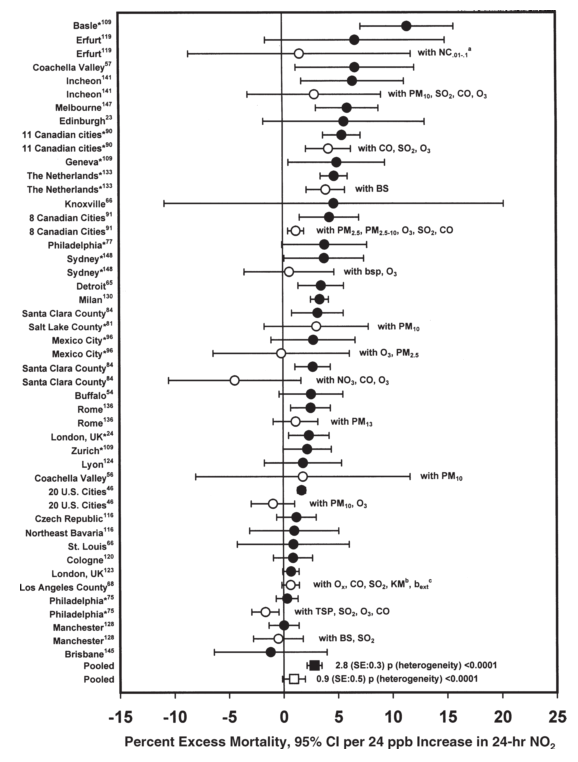
\includegraphics[scale=0.8]{short_term_no2_meta}
\caption{Percent excess mortality}
\label{fig:short_term_no2_meta}
\end{figure}

To summarise, the research that has been conducted so far, with the data available, suggests that the effects of long-term pollution are a more important determinant of poor health than that of short-term exposure. However the studies are limited and lack detail sometimes in areas which potentially alter their conclusions. Kloog et al. and \gls{comeap} looked at \gls{pm25} (though perhaps this is sensible given the discussion in Section \ref{subsec:anoverview}), and Beverland et al. only considered black smoke. There were limitations of spatial and temporal resolution of the pollution data and subsequent linkage in the three of the studies. Often large data-sets cannot consider all important details. Definitions of how long 'long-term' and how short 'short-term' are could also be an influence on conclusions drawn. Short-term is taken to be around 3 days exposure, but this could be missing hyper-short term exposure, such as a subject spending an hour cycling down a busy road and perhaps triggering hospital admission for breathing difficulties. With better air quality data and more in-depth better information on where people spend their time (and therefore are exposed) it might be possible to overcome these issues, however the data to do this does not presently exist for epidemiologists to use.

It is important to consider both the rapid effects of air pollution exposure e.g. pathways without hours of exposure \textbf{and} the chronic effects of sustained exposure (\cite{Brook2010}).

It seems that short-term, hyper-short-term and long-term exposure are all important in understanding the health effects of air pollution. Thus studies that are able to consider large population exposures (but with information on individuals available), and on these varying time--scales are required. This issue of improving linkage between air quality and exposure has evolved over time. The next section reviews the various methods that have been used in the past to link air quality and exposure time -- what I term 'static exposure studies'. Studies that make use of various different metrics for air quality, but do not take into account the movement of people. Dynamic exposure studies are then described -- those that take this movement and other factors into account.

%This has just come out about short-term and irregular heart-beats: \url{http://www.theguardian.com/environment/2014/jun/05/air-pollution-linked-to-irregular-heart-beat-study-finds?CMP=twt_fd}

%Short-term health effects in the 'Oxford Street' study by \cite{McCreanor2007}.
\newpage
%%%%%%%%%%%%%%%%%%%%%%%%%%%%%%%%%%%
%%% Static exposure studies
%%%%%%%%%%%%%%%%%%%%%%%%%%%%%%%%%%%

\section{Static exposure \& health studies}
\label{sec:staticexposurehealth}

The methods of estimating individual and population level exposure to air pollutants (and from this data the impact on health) has evolved over time; better data has become available, computer modelling has become more complex (facilitated by more powerful computers), and more accurate methods have been employed. This section of the PhD takes an overview of the methods of exposure assessment that I term 'static exposure' studies. That is, the subjects to which the air pollution is being attributed do not move between environments and their exposure is calculated (normally) at their residential address. In addition the temporal and spatial granularity of the air quality data is often (in my opinion) of low or insufficient quality.

This section is split into the following categories:

\begin{itemize}
\item Large area exposure
\item Monitoring stations
\item Proximity to roads
\item Dispersion modelling
\item Land-use regression
\end{itemize}

Due to a large literature base, these sections draw on key texts for each section as examples of the approach being described. By considering the issues and problems with these studies, I suggest that they over-simplify exposure in different ways, justifying the use of dynamic exposure models (which are explained and then thoroughly reviewed in Section \ref{sec:dynamicexposurehealth}, '\nameref{sec:dynamicexposurehealth}').

%%%%%%%%%%%%%%%%%%%%%%%%%%%%%%%%%%%
%%% Large area exposure
%%%%%%%%%%%%%%%%%%%%%%%%%%%%%%%%%%%

\subsection{Large area exposure}
\label{subsec:largearea}

Large area exposure studies are studies which, as the title suggests, attribute exposure to subjects over a large spatial area. This might be at the level of a city, a county or even continent. The well known Global Burden of Disease studies (discussed briefly in \ref{subsec:longtermvshortterm}) are classic examples of this approach. For the global burden of \gls{pm25} (chosen due to it's strong links in the literature with poor health) in 1990 and 2005 an annual average layer of air pollution was modelled for the entire world at 0.1\textsuperscript{o} x 0.1\textsuperscript{o} spatial resolution (shown in figure \ref{fig:globalburdenpm25}).

\begin{figure}[H]
\centering
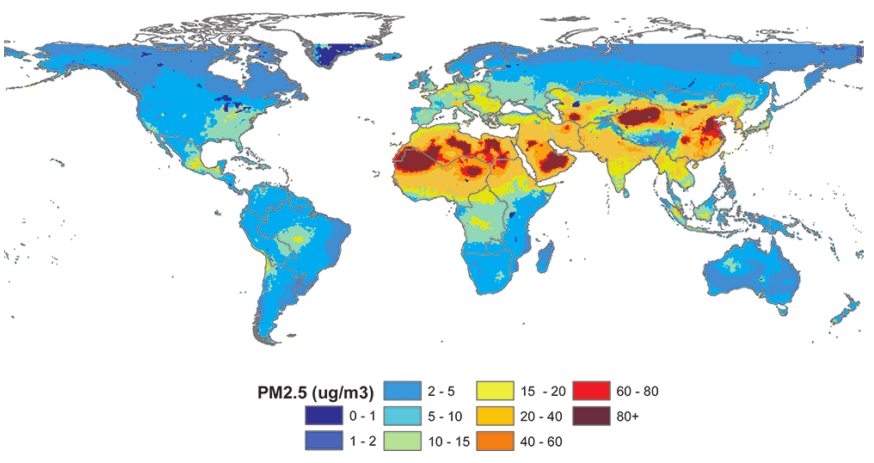
\includegraphics[scale=0.6]{global_burden_pm25}
\caption{Estimated 2005 annual average \gls{pm25} concentrations (ug/m\textsuperscript{3})}
\label{fig:globalburdenpm25}
\end{figure}

To generate this worldwide layer of \gls{pm25} satellite derived observations of Aerosol Optical Depth (\gls{aod}) were used (\cite{Brauer2012}). When this work was undertaken this was not a particularly common approach for exposure assessment, mainly due to lack of understanding in this new field and the resolution being relatively low, however as new earth observation satellites are launched the approach is gaining in popularity (\cite{VanDonkelaar2015}, \cite{Hoek2017}).

The resulting health conclusions/estimations from large scale exposure models are discussed in Section \ref{subsec:longtermvshortterm}, here we focus on limitations with the methods. Firstly, ambient concentrations are assigned to the entire population of the grid cells i.e. no micro-environmental modelling is undertaken to allow for the time that people spend indoors, or indeed in any other environment. Secondly, modelling at 0.1\textsuperscript{o} x 0.1\textsuperscript{o} resolution means much of the spatial variation in concentrations is lost i.e. there is a great deal of small scale variation in concentrations within the area which are not being included. To elucidate further, we know from Section \ref{subsec:urbanenvironments} that people are concentrated in urban environments rather than distributed evenly across countries and continents, and that within these environments levels of pollution are higher than outside of them, primarily due to emissions from combustion engines (Section \ref{subsec:trafficpollution}). Taking London as an example, the city is approximately 50 km wide, yet a degree of longitude is approximately 113 km wide, meaning that (in this oversimplification example) the exposure attributed to someone living in the middle of the Kent downs where are much fewer sources of \gls{pm25} is the same as someone living in the centre of London, where the sources of \gls{pm25} are more frequent. The authors argue that as the population data is of a similar scale this does not matter so much, however by not being able to take account of these urban environments, or at least not at an adequate scale, exposure may be incorrectly attributed. Though to what degree it is hard to know. Thirdly, the lack of temporal resolution to the air quality layer is a problem. As was briefly explored in the sections on traffic-generated pollution (\ref{subsec:trafficpollution}) and meteorology (\ref{subsec:meteorology}), air quality varies by hour, week, days, months, seasons etc.

Studies of similar scales include \cite{Silva2013} who combined 14 atmospheric chemistry and meteorological models to attribute annual average \gls{pm25} exposure to the worlds population on a scale of 0.5\textsuperscript{o} by 0.5\textsuperscript{o} degrees resolution, and \cite{Boldo2011} who modelled \gls{pm25} at a resolution of 18 km by 18 km (figure \ref{fig:gspain_pm25_grid}) to cover the country of Spain (both approaches then used concentration-response functions to estimate mortality).

\begin{figure}[H]
\centering
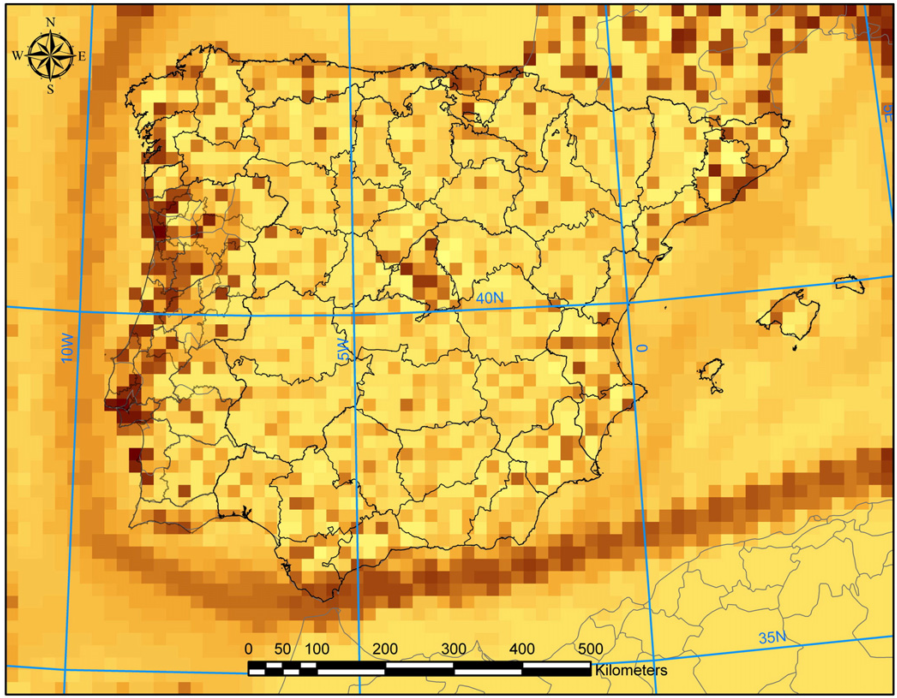
\includegraphics[scale=0.6]{spain_pm25_grid}
\caption{Grid squares used for \gls{pm25} exposure}
\label{fig:gspain_pm25_grid}
\end{figure}

It should be stated at this point, that the criticism levelled at these papers is symptomatic of many studies discussed in the next sections of this report. However doing so is often a little unfair. The researchers were in most cases doing the best work that technology, available data, or indeed time or known methods allowed them to do. As the discussion moves into reviewing further literature in Section \ref{sec:dynamicexposurehealth} (\nameref{sec:dynamicexposurehealth}), the suggestion is that methods can now be improved beyond this position.

%%%%%%%%%%%%%%%%%%%%%%%%%%%%%%%%%%
%%% Monitoring stations
%%%%%%%%%%%%%%%%%%%%%%%%%%%%%%%%%%

\subsection{Monitoring stations}
\label{subsec:monitoringstation}

%% What is a monitoring station
The term 'air quality monitoring station' or simply 'monitoring station', within the context of this field of research, typically refers to a static cabin or large metal box which houses a number of instruments that measure various air pollutants and meteorological conditions at specific time intervals. A typical station is shown in Figure \ref{fig:monitoring_station} from \url{www.londonair.org.uk}.

\begin{figure}[H]
\centering
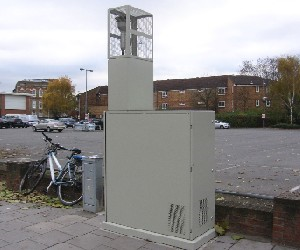
\includegraphics[scale=1.3]{monitoring_station}
\caption{A typical monitoring station}
\label{fig:monitoring_station}
\end{figure}
%% Often used for regulatory purposes. Sometimes statutory.

In the UK monitoring stations were first set-up after the introduction of the Clean Air Act in 1956, and the numbers of stations, locations, the accuracy, time resolution and numbers of pollutants that are monitored has changed incrementally since then. The last change in organisation of the sites came in 1998, when the then Department of Environment established the Automatic Urban and Rural Network (\gls{aurn}), bringing together many sub-networks to form the most comprehensive automatic national monitoring network in the country, made up of 127 sites (\cite{DEFRA2011a}). The data collected from the sites is used for policy and legislative purposes, including reporting to the \gls{eu} (long may this continue), however as the data is routinely and automatically collected over long periods of time the outputs have been a popular dataset for researchers too. \cite{Mayer1999} presents a good example of the temporal variability of data that can be collected such as \gls{no}, \gls{no2}, \gls{o3} and \gls{nox} at an urban air quality station in Stuttgart, Germany (and then subsequently linked to populations for estimating exposure).

One of the most highly cited research articles where data of this nature was used is in the paper '\textit{An association between air pollution and mortality in six US cities}' by \cite{Dockery1993}. In this study air pollution exposure was linked to 8111 adults over six cities in the\gls{us} from six monitoring sites (one in each city) in the form of annual average concentrations. Each station measured \gls{pm25} and \gls{pm10} (PM$_{15}$ before 1984). After adjusting for smoking and other risk factors, significant associations between air pollution and mortality were found.  Studies that also used monitoring stations in a similar way include \cite{Atkinson2010} who did a time-series analysis of London hospital admissions using data from a background monitoring site (\gls{pm10}, \gls{pm25}, PM$_{10-2.5}$) and found associations between various pollutants and health outcomes outcomes such as daily mortality (particular for cardiovascular), and then \cite{Samoli2005} who as part of the APHEA Multi-city Project took monitoring site data for 22 \gls{eu} cities and found links with mortality from the air quality data of these stations.

The main question with this type of approach however is that of temporal and spatial variability, and resolution - can the data from a monitoring site be an appropriate measure of exposure for someone who, in many examples, may live miles from the monitoring site. Certainly the studies that have tried to address whether this is appropriate or not have found poor correlation between the two. \cite{Cyrys2008} found that '\textit{the use of a single monitoring station in long-term epidemiological studies must be insufficient to attribute accurate exposure levels of \gls{pnc}s to all study subjects}' i.e. it might work for some people but not for all. Although it's worth noting here that they believe that the monitoring stations do an accurate job of reflecting temporal variability, particularly for ultra-fine particles. Just not the spatial variability. \cite{Goldstein197747} broadly agree, they found in New York that '\textit{the procedure of using one aerometric station to represent the daily fluctuations of air pollution throughout the large metropolitan area of New York City risks the use of an unreliable or invalid measure of the short term variation in air pollution'}. So their message is slightly different, in that their research did not assesses how valid it would be as a measure of long-term variation, but they did conclude it is poor for short-term (whether long-term or short-term exposure to poor air quality is more important as a measure is discussed in Section \ref{subsec:longtermvshortterm}, \nameref{subsec:longtermvshortterm}). \cite{Willocks2012} in Scotland extended two existing studies of the relationships between air quality at monitoring sites and cardiovascular disease, and more broadly reflected on the difficulties in conducting this sort of study, and found \textit{"no consistent associations [...] between \gls{pm10} concentrations and cardiovascular hospital admissions"}. 

Whether this mis-classification of exposure to pollutants varies between pollutants and height from the ground was considered by \cite{Restrepo2004} who took data from three different monitoring stations (15m above ground) and compared it to data from a van which contained similar equipment but which was parked at three different locations and with the equipment inlets at 4m above ground.The stations showed good agreement between themselves, but not with the ground-level (van) data. \gls{pm25} was closest matched, for ozone the ground level concentrations were generally lower, and for \gls{no2} the concentrations at ground level were over twice as high as those at the monitoring stations.\\ 

To conclude, using data from monitoring stations as a proxy for estimating exposure for large populations over many kilometres does not seem to accurately reflect individuals exposure. The studies above tended to look at the correlation between a subjects residential address and the monitoring station, meaning that there is then the additional complicating factor that people do not spend all of their time at their home. Whilst the data is certainly easily obtained and the temporal resolution makes it attractive for time-series studies, the lack of spatial variability and lack of any micro-environmental modelling or understanding of where subjects actually spend their time mean that this approach is simplistic.

%%%%%%%%%%%%%%%%%%%%%%%%%%%%%%%%%%
%%% Proximity to roads
%%%%%%%%%%%%%%%%%%%%%%%%%%%%%%%%%%
\subsection{Proximity to roads}
\label{subsec:proximitytoroads}

The use of subject's address data, and then a calculation of the number of roads (and sometimes traffic density on those roads), is another proxy measure of exposure that has been used to consider exposure to air quality and links between this and poor health. One of the most highly-cited papers in this area is by \cite{Gauderman2007}  who specifically looked at whether living near to major roadways in California had an impact on lung-function growth of children between the ages of 10 and 18. In the study 3677 children were regularly monitored for 8 years and yearly lung-function tests were completed, which were then considered alongside their home address and the distance to the nearest freeway. They found that proximity to freeway traffic is associated with substantial deficits in lung function (which became less pronounced the further the child lived from the freeway). Similar studies include those by \cite{Janssen2001} and \cite{Rose2009}, although both do not go as far as to make conclusions of health outcomes, they focus on the method of exposure estimation by road density. A wider-review of studies in this area was also undertaken by the \cite{HPotHEoT-RA2010} in the report '\textit{Traffic-related air pollution: a critical review of the literature on emissions, exposure, and health effects}'.

The presumption of this type of study is that the air quality the subjects are exposed to during normal day-to-day activities is strongly correlated to the air quality at their home, and that the air quality at their home is strongly correlated with the number of freeways within certain buffer distances of their home. These studies also mostly look at annual average traffic flows or similar, and therefore seem to not take account of variation in road use and therefore pollution levels. Indeed, combining these issues only exasperates the uncertainty, for example road flows are mostly higher during the morning and evening rush-hours, when children between 10 and 18 are likely on their way to school or already at school i.e. not at home as the model presumes. They also don't consider the time a subject is not at their home, or any other micro-environment. 

%%%%%%%%%%%%%%%%%%%%%%%%%%%%%%%%%%%
%%% Dispersion modelling
%%%%%%%%%%%%%%%%%%%%%%%%%%%%%%%%%%%

\subsection{Dispersion modelling}
\label{subsec:dispersionmodelling}

To better bridge this distance between where exposure is occurring (often presumed to be the subject's household) and where the exposure is being estimated or measured (such as a monitoring site) modelling can be used to create maps or layers of varying resolution for the area that the study or subjects are based in.

Dispersion modelling is a way of simulating the movement of emissions through the atmosphere using mathematical equations with input variables such as wind speed, wind direction, air temperature and street geography (\cite{EnvironmentalProtectionAgency2008}). By doing this at different scales (country-wide, city-wide, individual streets) it is possible to create pollution maps and to then associate the pollutant values at those places with the people who live there - estimating their exposure - and possibly linking this to health effects if data is available.

% --------Now talk here about the Maroko paper as that basically is a paper which says proximity analysis is bad and that dspersion is better. Uses environmetnal justice as the outcomes.

\cite{Maroko2012}, in studying environmental justice in New York City (\gls{usa}) compared the differences between using a proximity analysis technique (similar to \ref{subsec:proximitytoroads} - proximity to roads) and a dispersion model of \gls{pm25}. Their hypothesis was that minority populations were more likely to be located in areas of poor air quality, and that proximity analysis may under-represent this problem. Figure \ref{fig:maroko_stack_proximity} shows tax-lots within 1\slash4 mile of the point stacks upon which the initial exposure analysis (and subsequent assessment of over-representation of minorities) was completed. 

\begin{figure}[H]
\centering
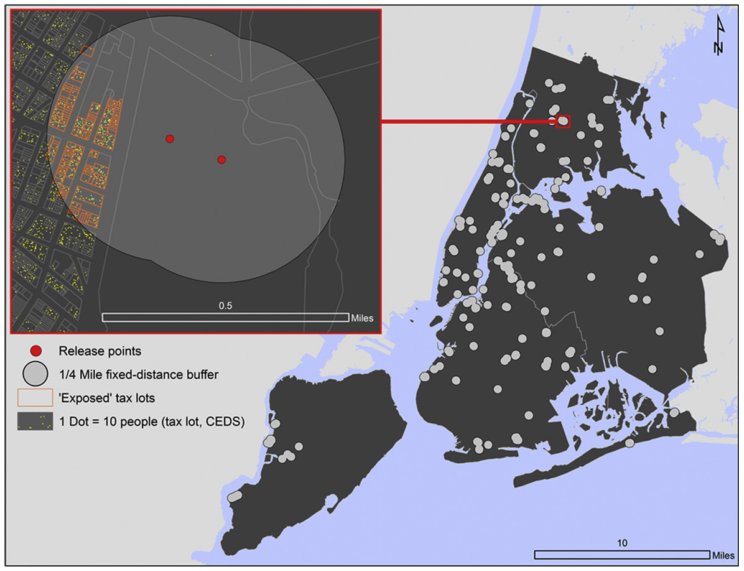
\includegraphics[scale=0.75]{maroko_stack_proximity}
\caption{Proximity analysis to \gls{pm25} point sources}
\label{fig:maroko_stack_proximity}
\end{figure}

Figure \ref{fig:maroko_dispersion_map} then shows the same area, but now using dispersion modelling.

\begin{figure}[H]
\centering
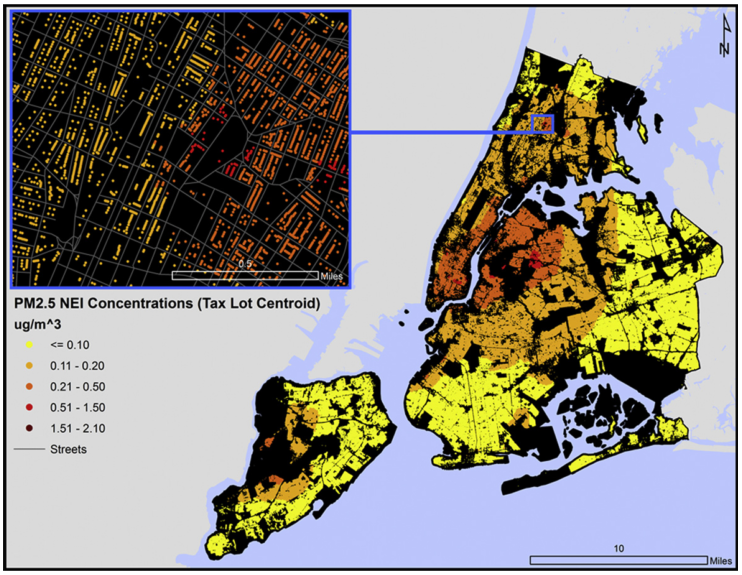
\includegraphics[scale=0.75]{maroko_dispersion_map}
\caption{\gls{pm25} estimates from dispersion modelling allocated to tax--lots}
\label{fig:maroko_dispersion_map}
\end{figure}

As is clear to see, the dispersion modelling approach provides a greater degree of spatial detail and clarity. Using this second approach to exposure assessment, they were able to identify that Latino groups in the Bronx and Brooklyn were being dis-proportionally exposed to higher levels of poor air quality than other ethnic groups, which was not evident from the proximity analysis approach. Also using a dispersion model but in London, \cite{Tonne2010} calculated the London annual average concentrations for 2001 and 2005 (pre and post the Congestion Charging Scheme (\url{http://www.tfl.gov.uk/modes/driving/congestion-charge})) for \gls{no2} and \gls{pm10} on a 20m x 20m grid, and then using this aggregated the data to Ward level (shown in Figure \ref{fig:tonne_wards_dispersion}).

\begin{figure}[H]
\centering
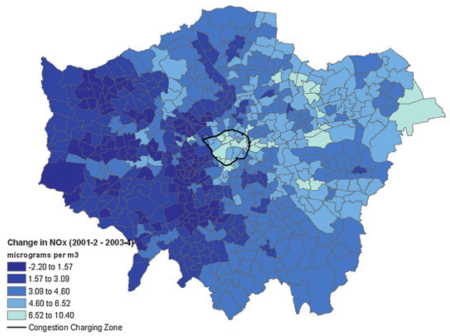
\includegraphics[scale=1]{tonne_wards_dispersion}
\caption{Map of \gls{nox} change at Ward level between 2001 and 2005, based on dispersion modelling}
\label{fig:tonne_wards_dispersion}
\end{figure}

The association between this change in concentration and respiratory hospital admissions was then calculated, although no conclusive relation was found.

Both of these studies (\cite{Maroko2012} and \cite{Tonne2010}) seem to be a step in the right direction for improving estimates of exposure as they provide air quality data at a higher resolution than many of the studies that were considered earlier, however there are still concerns that they misclassify exposure by not adequately taking account of temporal variation in air quality, where the subjects are actually spending their time, and the micro-environmental aspects.

%%%%%%%%%%%%%%%%%%%%%%%%%%
%%% Land use regression
%%%%%%%%%%%%%%%%%%%%%%%%%%

\subsection{Land-use regression}
\label{subsec:landuseregression}

Land-use regression (\gls{lur}) maps of air quality, and linking the concentrations from these maps to subjects for health studies, was first undertaken as part of the 'Small Area Variations In Air quality and Health' (SAVIAH) study by \cite{Briggs1997}. Land-use regression models combine monitoring of air pollution at a small number of locations, and then develop models using predictor variables normally obtained through geographic data i.e. proximity of roads, land-use, number of nearby buildings, heights of buildings etc. These models are then applied to un-sampled locations in the study area, and concentration values generated using the characteristics of the new location.

A review of the use of \gls{lur} modelling for outdoor air concentration values was published by \cite{Hoek2008}. They found that the models could be applied relatively successfully to model annual mean concentrations in various geographical locations, for various pollutants including \gls{no2}, \gls{nox}, \gls{pm25} and \gls{vocs}, and that the method was better than other geo-statistical methods such as kriging and dispersion methods. However the models were not as effective when a finer temporal scale was required or desired. \cite{Dons2013} in a study accross Flanders (Belgium) used aetholometers with a 5-minute resolution to measure black carbon at 63 locations continuously for seven days. When they compared these values to a \gls{lur} model they concluded similarly to Hoek, that existing \gls{lur} models were not adequately representing the exposure of the local population, due to the lack of temporal variability in the model. Dons followed this through by attempting to develop an hourly \gls{lur} model; with some success. The R$^{2}$of their models varied between 0.15 and 0.79 according to the time of day and the variables used as input.

In the recent paper by \cite{Pedersen2013}, which is an output from the ESCAPE (European Study of Cohorts for Air Pollution Effects) project, a \gls{lur} model was generated for 12 European countries, and then temporally adjusted using hourly profiles from nearby monitoring sites (to try to introduce temporal variability that has been lacking from this approach as noted by Hoek). Links between the concentrations at the maternal address of 74,178 women, who had singleton deliveries between 1994 and 2011, were then examined. They found that a 5 $\mu \text{g m}^{-3}$ increase in concentrations of \gls{pm25} during pregnancy was associated with an increased risk of low birthweight.\newline

To summarise, \gls{lur} models are being used for health studies, and conclusions between health outcomes and air pollution are being drawn, however there are similar problems with the exposure estimates as in many of the other previous static exposure estimate methods, including that there is no estimation of the amount of time that people spend away from their home and the pollutants and concentrations that they are exposed too i.e. how much time did the mothers in the ESCAPE study actually spent at their maternal address? Studies using \gls{lur} models also don't tend to conduct any micro-environmental modelling of the time that subjects spend indoors or in transport, and the methods behind the temporal variability might be considered further i.e. is using a nearby monitoring stations daily variation sufficient to reflect the daily variation at the address point. A further more generic problem with using \gls{lur} models for exposure assessment is that they require monitoring to have been conducted in the area that the model is proposed to be used in (and setting up a dense enough network of monitors to provide accurate model results is expensive and time--consuming).

%%%%%%%%%%%%%%%%%%%%%%%%%%
%%% The death of static exposure studies
%%%%%%%%%%%%%%%%%%%%%%%%%%

\subsection{Progressing on from static exposure studies}
\label{subsec:progressing_from_static}

In the review article \textit{"Spatio-temporal epidemiology: principles and opportunities"}, \cite{Meliker2011} discuss how estimating exposure is a rapidly evolving field, and how geographic information sciences, computing power and big data have started to overcome the issues that traditional spatio-temporal epidemiology has often struggled with. As air quality modelling efforts, and linked static exposure assessments, are producing ever-more spatially and temporally accurate estimates of pollutants, spatial analysis techniques and big data are stepping in to compliment these fields by incorporating the mobility of the population in ways not previously possible.

\begin{quote}
"We expect exposure assessments to increasingly incorporate space--time dynamics in particular mobility and environmental contaminants, such that it becomes commonplace in the near future" \cite{Meliker2011}
\end{quote}

The following section titled 'Dynamic exposure and health studies', looks at these new type of studies that explicitly seek to take account of the movement of individuals through different environments, and their exposure in those environments.

